\documentclass{apcalc}
\title{Unit 6: Integration and Accumulation of Change}
\author{Paul Wang}
\date{November 2026}
\volume{Study Guide 6 of 10 (topics 6.1--6.14)}
\shorttitle{Unit 6 --- Study Guide}
\begin{document}
\maketitle

\begin{abstract}
Unit 6 is the heaviest unit in the course (15--20\% of the multiple-choice section) and the one every later unit leans on. It builds the definite integral as a limit of Riemann sums, connects it to derivatives through both parts of the Fundamental Theorem of Calculus, and develops the BC techniques: substitution, integration by parts, partial fractions and improper integrals. Free-response questions test it through Riemann sums from tables, accumulation functions defined by $\int_a^x f(t)\,dt$ with a graph of $f$, and net change. This guide states the unit in fourteen rules (R6.1--R6.14) across six sections. The \emph{Unit 6 Practice Set} uses the same section numbers.
\end{abstract}
\keywords{accumulation, Riemann sum, trapezoidal sum, definite integral, Fundamental Theorem of Calculus, accumulation function, antiderivative, substitution, integration by parts, partial fractions, improper integral.}

\section*{Router}
\begin{router}
table of rates, ``approximate the total'' & left, right, midpoint or trapezoidal sum with the given (uneven) widths & R6.2 \\
$\lim_{n\to\infty}\sum f(x_k)\Delta x$ & rewrite as $\int_a^b f(x)\,dx$: read $\Delta x$ and $x_k$ & R6.3 \\
$\frac{d}{dx}\int_a^{g(x)}f(t)\,dt$ & $f(g(x))\,g'(x)$ & R6.4 \\
$g(x)=\int_a^x f(t)\,dt$ with a graph of $f$ & $g'=f$, $g''=f'$; values are signed areas & R6.5 \\
``amount at time $b$'' & initial amount $+\int_a^b(\text{rate})\,dt$ & R6.7 \\
an inside function whose derivative is present & $u$-substitution; change the limits & R6.9 \\
improper fraction, or $\frac{1}{x^2+bx+c}$ & long division / complete the square & R6.10 \\
$x^ne^x$, $x\sin x$, $x^n\ln x$, $e^x\sin x$ & integration by parts & R6.11 \\
$\frac{\text{linear}}{(x-a)(x-b)}$ & partial fractions & R6.12 \\
$\infty$ as a limit, or a vertical asymptote in $[a,b]$ & improper integral: write it as a limit & R6.13 \\
\end{router}

\section{Accumulation and Riemann sums (6.1--6.3)}

\begin{rulebox}{R6.1}{Accumulation}
The area between the graph of a rate $r(t)$ and the $t$-axis over $[a,b]$ is the net amount accumulated. Units: (units of $r$) $\times$ (units of $t$). Area below the axis counts as negative (a net decrease).
\end{rulebox}

\begin{rulebox}{R6.2}{Riemann and trapezoidal sums}
With subintervals of widths $\Delta x_k$: left sum uses left endpoints, right sum right endpoints, midpoint sum midpoints; the trapezoidal sum averages left and right: $\sum\frac{f(x_{k-1})+f(x_k)}{2}\Delta x_k$. Widths may be unequal in a table: multiply each height by its own width. If $f$ is increasing, a left sum underestimates and a right sum overestimates (reverse for decreasing). If $f$ is concave up, the trapezoidal sum overestimates (and the midpoint sum underestimates).
\end{rulebox}

\begin{example}{a table with unequal widths}
\begin{center}\small\begin{tabular}{|c|c|c|c|c|}\hline $t$ (hours) & 0 & 2 & 5 & 6\\\hline $r(t)$ (liters/hour) & 10 & 14 & 20 & 17\\\hline\end{tabular}\end{center}
Trapezoidal sum for $\int_0^6 r(t)\,dt$: $\frac{10+14}{2}(2)+\frac{14+20}{2}(3)+\frac{20+17}{2}(1)=24+51+18.5=93.5$ liters. Right sum: $14(2)+20(3)+17(1)=105$. \answer{trapezoid 93.5 L.}
\end{example}

\begin{rulebox}{R6.3}{The definite integral as a limit}
$\displaystyle\int_a^b f(x)\,dx=\lim_{n\to\infty}\sum_{k=1}^n f(x_k)\,\Delta x$ with $\Delta x=\frac{b-a}{n}$ and $x_k=a+k\Delta x$ (right endpoints). To convert a given limit, identify $\Delta x$ (the factor outside), then $a$ and the function: $\lim\sum_{k=1}^n\left(2+\frac{3k}{n}\right)^2\frac3n=\int_2^5x^2\,dx$ (or $\int_0^3(2+x)^2dx$).
\end{rulebox}

\section{Accumulation functions and the FTC (6.4--6.6)}

\begin{rulebox}{R6.4}{Fundamental Theorem, part 1}
If $f$ is continuous, $\dfrac{d}{dx}\displaystyle\int_a^x f(t)\,dt=f(x)$. With a variable upper limit $u(x)$: $\dfrac{d}{dx}\displaystyle\int_a^{u(x)}f(t)\,dt=f(u(x))\,u'(x)$. With both limits variable, split at a constant.
\end{rulebox}

\begin{rulebox}{R6.5}{Analyzing $g(x)=\int_a^x f(t)\,dt$}
$g(a)=0$; $g'(x)=f(x)$; $g''(x)=f'(x)$. So $g$ increases where the graph of $f$ is above the axis, has a relative max where $f$ crosses from $+$ to $-$, and is concave up where $f$ is increasing. Values of $g$ come from signed areas: $g(x)=$ (area above) $-$ (area below) between $a$ and $x$; for $x<a$, $g(x)=-\int_x^a f$.
\end{rulebox}

\begin{example}{accumulation from a graph}
\begin{center}
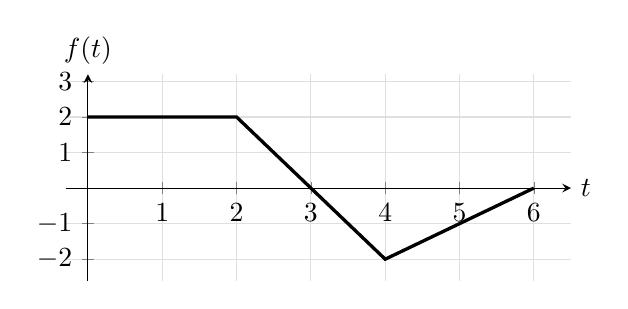
\begin{tikzpicture}
\begin{axis}[width=8cm,height=4.2cm,axis lines=middle,xmin=-0.3,xmax=6.5,ymin=-2.6,ymax=3.2,xtick={1,...,6},ytick={-2,-1,1,2,3},xlabel={$t$},ylabel={$f(t)$},grid=major,grid style={gray!25},
 every axis x label/.style={at={(ticklabel* cs:1)},anchor=west},every axis y label/.style={at={(ticklabel* cs:1)},anchor=south}]
\addplot[very thick] coordinates{(0,2) (2,2) (4,-2) (6,0)};
\end{axis}
\end{tikzpicture}
\end{center}
Let $g(x)=\int_0^x f(t)\,dt$ for the graph shown. $g(2)=4$ (rectangle), $g(3)=4+1=5$, $g(4)=5-1=4$, $g(6)=4-2=2$. $g$ has its maximum at $x=3$, where $f$ changes from positive to negative; $g$ is concave up on $(4,6)$, where $f$ increases. \answer{$\max g=g(3)=5$.}
\end{example}

\begin{rulebox}{R6.6}{Properties of definite integrals}
$\int_a^a f=0$; $\int_b^a f=-\int_a^b f$; $\int_a^b f+\int_b^c f=\int_a^c f$; integrals are linear. If $f$ is odd, $\int_{-a}^a f=0$; if even, $\int_{-a}^a f=2\int_0^a f$. Use geometry (rectangles, triangles, semicircles) when the integrand is a known shape: $\int_{-3}^3\sqrt{9-x^2}\,dx=\frac{9\pi}{2}$.
\end{rulebox}

\section{Antiderivatives and the FTC, part 2 (6.7--6.8)}

\begin{rulebox}{R6.7}{Fundamental Theorem, part 2 and net change}
If $F'=f$ on $[a,b]$ with $f$ continuous, then $\displaystyle\int_a^b f(x)\,dx=F(b)-F(a)$. Net change: $F(b)=F(a)+\int_a^b F'(x)\,dx$. This is the most-used sentence on the free response: ``amount at time 4 $=$ amount at time 0 $+\int_0^4$(rate in $-$ rate out)$\,dt$.''
\end{rulebox}

\begin{rulebox}{R6.8}{Basic antiderivatives}
$\int x^n\,dx=\frac{x^{n+1}}{n+1}+C$ ($n\neq-1$); $\int\frac1x\,dx=\ln|x|+C$; $\int e^x\,dx=e^x+C$; $\int a^x\,dx=\frac{a^x}{\ln a}+C$; $\int\sin x\,dx=-\cos x+C$; $\int\cos x\,dx=\sin x+C$; $\int\sec^2x\,dx=\tan x+C$; $\int\sec x\tan x\,dx=\sec x+C$; $\int\frac{dx}{1+x^2}=\arctan x+C$; $\int\frac{dx}{\sqrt{1-x^2}}=\arcsin x+C$.
\end{rulebox}

\section{Substitution and algebraic techniques (6.9--6.10)}

\begin{rulebox}{R6.9}{$u$-substitution}
Choose $u$ as an inside function whose derivative appears (up to a constant). Write $du=u'(x)\,dx$, rewrite everything in $u$, integrate. For definite integrals, \emph{change the limits} to $u$-values (or back-substitute before evaluating).
\end{rulebox}

\begin{example}{substitution with new limits}
$\displaystyle\int_0^{2}x\,e^{x^2}\,dx$: $u=x^2$, $du=2x\,dx$, limits $0\to0$, $2\to4$: $\frac12\int_0^4e^u\,du=\frac12(e^4-1)$. \answer{$\frac{e^4-1}{2}$.}
\end{example}

\begin{rulebox}{R6.10}{Long division and completing the square}
If the numerator's degree is at least the denominator's, divide first: $\frac{x^2+1}{x+1}=x-1+\frac{2}{x+1}$. For $\frac{1}{x^2+bx+c}$ with no real roots, complete the square and use $\int\frac{du}{u^2+a^2}=\frac1a\arctan\frac ua+C$: $\int\frac{dx}{x^2+4x+13}=\frac13\arctan\frac{x+2}{3}+C$.
\end{rulebox}

\section{Integration by parts and partial fractions (6.11--6.12)}

\begin{rulebox}{R6.11}{Integration by parts (BC)}
$\int u\,dv=uv-\int v\,du$. Choose $u$ by LIATE (Log, Inverse trig, Algebraic, Trig, Exponential): $u$ is the first type present. For $x^ne^{x}$ repeat (or use the tabular method). For $e^x\sin x$, integrate by parts twice and solve for the integral.
\end{rulebox}

\begin{example}{by parts}
$\int x\cos x\,dx$: $u=x$, $dv=\cos x\,dx$, $du=dx$, $v=\sin x$: $x\sin x-\int\sin x\,dx=x\sin x+\cos x+C$.\par
$\int\ln x\,dx$: $u=\ln x$, $dv=dx$: $x\ln x-\int x\cdot\frac1x\,dx=x\ln x-x+C$.
\end{example}

\begin{rulebox}{R6.12}{Partial fractions (BC)}
For distinct linear factors: $\dfrac{px+q}{(x-a)(x-b)}=\dfrac{A}{x-a}+\dfrac{B}{x-b}$. Find $A$ by covering $(x-a)$ and substituting $x=a$ (Heaviside); same for $B$. Each piece integrates to a logarithm.
\end{rulebox}

\begin{example}{partial fractions}
$\displaystyle\int\frac{5x-1}{(x+1)(x-2)}\,dx$: $A=\frac{5(-1)-1}{-1-2}=2$, $B=\frac{5(2)-1}{2+1}=3$, so the integral is $2\ln|x+1|+3\ln|x-2|+C$.
\end{example}

\section{Improper integrals and choosing a technique (6.13--6.14)}

\begin{rulebox}{R6.13}{Improper integrals (BC)}
Infinite limit: $\int_a^\infty f=\lim_{b\to\infty}\int_a^b f$. Infinite discontinuity at $c$: split there and take one-sided limits. The integral converges if the limit is finite. Benchmarks: $\int_1^\infty\frac{dx}{x^p}$ converges iff $p>1$; $\int_0^1\frac{dx}{x^p}$ converges iff $p<1$. Write the limit: the scoring guide requires the limit notation.
\end{rulebox}

\begin{example}{an improper integral}
$\displaystyle\int_0^\infty xe^{-x}\,dx=\lim_{b\to\infty}\Big[-xe^{-x}-e^{-x}\Big]_0^b=\lim_{b\to\infty}\left(-\frac{b}{e^b}-\frac{1}{e^b}+1\right)=1.$ \answer{converges to 1.}
\end{example}

\begin{rulebox}{R6.14}{Selecting a technique}
Simplify first (expand, split the fraction, use an identity). Then: basic form $\to$ R6.8; inside function with its derivative $\to$ substitution; product of unlike types $\to$ parts; rational function $\to$ division, partial fractions or arctan. Check by differentiating your answer.
\end{rulebox}

\begin{trap}
$\int_{-1}^{1}\frac{dx}{x^2}$ is \emph{not} $-2$: the integrand has an infinite discontinuity at 0, and $\int_0^1\frac{dx}{x^2}$ diverges, so the integral diverges. Always scan $[a,b]$ for vertical asymptotes before using the FTC.
\end{trap}

\section{Common errors}
\begin{itemize}
\item Using one width for unequal subintervals in a table (R6.2).
\item Forgetting the chain factor $u'(x)$ in $\frac{d}{dx}\int_a^{u(x)}f$ (R6.4).
\item Treating an accumulation function's value as the height of $f$ instead of an area (R6.5).
\item Forgetting the initial amount in a net change problem (R6.7).
\item Keeping the $x$-limits after substituting $u$ (R6.9).
\item Using the FTC across a vertical asymptote (R6.13).
\end{itemize}

\end{document}
